\documentclass{article}
\usepackage[utf8]{inputenc}
\usepackage{xcolor}
\usepackage{url}
\usepackage{tikz}
\usepackage[nottoc]{tocbibind}
\usepackage{graphicx}
\usepackage[bottom]{footmisc}
\usepackage{tabularx}
\usepackage{graphicx}
\usetikzlibrary{positioning}
\usepackage{float}

\title{CSCE 479/879 Homework 1: Connected Architectures and Fashion MNIST}
\author{Derek DeBlieck, Sabrina Fowler, Grace Hecke, Abby Veiman}
\date{September 30, 2025}

\begin{document}

\maketitle

\begin{abstract}
    The problem for this assignment is to classify the Fashion MNIST data set. We want to find the best architecture for classifying these images. We also want to get some practice training and comparing models with different hyperparameters. Ultimately, the 8 trials we ran resulted in about the same level of accuracy on the test set. Also, our models with regularizers performed worse than their unregularized counterparts which suggests that an L2 regularizer is not optimal for this task.

    
% {\bf Do not cite any sources in the Abstract, since it is supposed to be self-contained (i.e., it might appear on its own without the References section).}
\end{abstract}

\section{Introduction}
\label{sec:intro}

For this assignment, we developed various architectures to classify the Fashion MNIST dataset. We created two main architecture structures, the first had one hidden layer with 128 nodes and the second had two hidden layers with 256 and 128 nodes respectively. We also varied our learning rates, trying 0.001 and 0.0005. We also tested the efficacy of an L2 regularizer. We tried all 8 combinations of these three binary options.

Overall, our models performed relatively similarly well, with accuracy on the test set ranging from 0.8669 to 0.8877. In general, the models using L2 regularization performed slightly less well than their unregularized counterparts.



% Here you should give a high-level overview of the problem you worked on for this assignment, your method(s), and a summary of your results.  


\section{Problem Description}

We were tasked with training a deep learning model to classify images from the fashion MNIST dataset. The data consists of images of various fashion items, labeled as t-shirt/top, trouser, pullover, dress, coat, sandal, shirt, sneaker, bag, and ankle boot. The data came from tensorflow-datasets, the training set consists of 60,000 images and the test set contains 10,000 images. In particular, the data comes to us as 28$\times$28 arrays with pixel intensities from 0-255.

This problem is interesting because it is similar to a problem we have worked on before in our Hackathons, classifying the handwritten digit MNIST data. However these images are more complicated than the digit images which should lead to a more complex model being necessary.

% Describe  the problem you worked on, including specifically what the learning problem was, how the data was formatted, where it came from, motivations for why this problem is interesting, etc. 

\section{Approaches}

Our approach to this problem involved setting up a general structure for our models and then varying the number of hidden layers, learning rates, and use of regularizer. Our general structure involved rescaling the pixel intensities to fall between 0 and 1 and flattening the 28$\times$28 arrays into a 1$\times$784 vectors. Then if we were using a regularizer that happened at this stage. Next, these were fed into our hidden layer(s), and then to a softmax layer with 10 nodes that served as our output layer. We also used a patience parameter of 3 to perform early stopping based on the validation loss. See below for figures demonstrating our neural network architectures.
\vspace{0.5in}

\begin{figure}[H]
\centering
\input{ArchitectureTikz.tex}
\caption{\bf{Architecture 1 with only a single hidden layer}}
\label{fig:arch1}
\end{figure}

\begin{figure}[H]
\centering
\tikzset{%
  every neuron/.style={
    circle,
    draw,
    minimum size=1cm
  },
  neuron missing/.style={
    draw=none,
    scale=4,
    text height=0.333cm,
    execute at begin node=\color{black}$\vdots$
  },
}

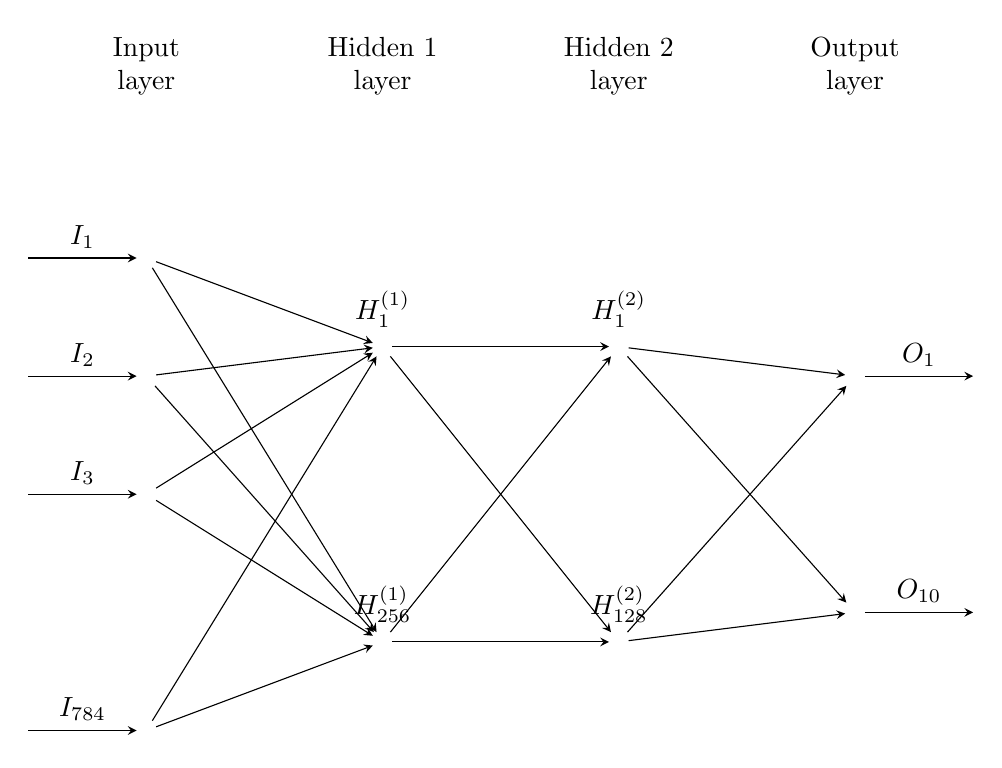
\begin{tikzpicture}[x=1.5cm, y=1.5cm, >=stealth]

% INPUT layer
\foreach \m/\l [count=\y] in {1,2,3,missing,4}
  \node [every neuron/.try, neuron \m/.try] 
    (input-\m) at (0,2.5-\y) {};

% FIRST HIDDEN layer
\foreach \m [count=\y] in {1,missing,2}
  \node [every neuron/.try, neuron \m/.try ] 
    (hiddenA-\m) at (2,2-\y*1.25) {};

% SECOND HIDDEN layer
\foreach \m [count=\y] in {1,missing,2}
  \node [every neuron/.try, neuron \m/.try ] 
    (hiddenB-\m) at (4,2-\y*1.25) {};

% OUTPUT layer
\foreach \m [count=\y] in {1,missing,2}
  \node [every neuron/.try, neuron \m/.try ] 
    (output-\m) at (6,1.5-\y) {};

% INPUT labels
\foreach \l [count=\i] in {1,2,3,{784}}
  \draw [<-] (input-\i) -- ++(-1,0)
    node [above, midway] {$I_{\l}$};

% Hidden labels
\foreach \l [count=\i] in {1,{256}}
  \node [above] at (hiddenA-\i.north) {$H^{(1)}_{\l}$};

\foreach \l [count=\i] in {1,{128}}
  \node [above] at (hiddenB-\i.north) {$H^{(2)}_{\l}$};

% Output labels
\foreach \l [count=\i] in {1,{10}}
  \draw [->] (output-\i) -- ++(1,0)
    node [above, midway] {$O_{\l}$};

% Connections: input -> hiddenA
\foreach \i in {1,...,4}
  \foreach \j in {1,...,2}
    \draw [->] (input-\i) -- (hiddenA-\j);

% Connections: hiddenA -> hiddenB
\foreach \i in {1,...,2}
  \foreach \j in {1,...,2}
    \draw [->] (hiddenA-\i) -- (hiddenB-\j);

% Connections: hiddenB -> output
\foreach \i in {1,...,2}
  \foreach \j in {1,...,2}
    \draw [->] (hiddenB-\i) -- (output-\j);

% LAYER labels
\foreach \l [count=\x from 0] in {Input, Hidden 1, Hidden 2, Output}
  \node [align=center, above] at (\x*2,2.8) {\l \\ layer};

\end{tikzpicture}

\caption{\bf{Architecture 2 with a two hidden layers}}
\label{fig:arch2}
\end{figure}




% Summarize the approach(es) you used to solve this problem, particularly focusing on the architectures you used ({\bf use figures describing layers and their sizes}), justifying all design decisions. 

\section{Experimental Setup}
We used the fashion MNIST dataset; we flattened each 28x28 image into a single vector with 784 features.  We tested two different neural network architectures: the first contained only a single hidden layer with 128 nodes, while the second consisted of two hidden layers.  The first of these hidden layers contained 256 nodes while the second contained 128 nodes. The Adam optimizer was used during model training, which used categorical cross-entropy as a loss function.  The Adam optimizer was used during training.  Additionally, we employed early stopping with a patient interval of 3 and a batch size of 32.  For each architecture, we trained models using a learning rate of 0.001 and 0.0005 additionally trained a model using $L_2$-regularization and a model without regularization.  This gives us a total of 8 trained models (2 architectures, $L_2$-regularization or no regularization, and 2 learning rates).


% Describe the setup of your experiments  in sufficient detail for the reader to reproduce them.  Include data sources, preprocessing used,  hyperparameter values used ({\bf use a table}), performance measures used, other relevant items (e.g., cross-validation).

\section{Experimental Results}
\label{sec:results}
Please see the table below for a summary of results.  Based on test accuracy, we found that the architecture with two hidden layers, a smaller learning rate, and no $L_2$-regularization was most accurate with the smallest generalization error.  However, the difference between these models was relatively small.  All models performed reasonably well, which we should expect for a relatively simple classification problem.

\begin{table}[H]
    \centering \caption{Summary of Model Architectures and their Performance}
    \begin{tabular}{|p{1.5cm}|p{1.3cm}|c|p{1.5cm}|p{1.3cm}|c|} \hline
      Hidden Layers   &  Learning Rate & Regularizer & Validation Accuracy & Test Accuracy & Generalization Error \\ \hline
    128 & 0.001 & n/a & 0.8938 & 0.8832 & 0.117 $\pm$ 0.006 (95\% CI) \\
    128 & 0.001 & L2 & 0.8800 & 0.8675 & 0.132 $\pm$ 0.007 (95\% CI) \\
    128 & 0.0005 & n/a & 0.9010 & 0.8840 & 0.116 $\pm$ 0.006 (95\% CI) \\
    128 & 0.0005 & L2 & 0.8873 & 0.8695 & 0.131 $\pm$ 0.007 (95\% CI) \\
    256, 128 & 0.001 & n/a & 0.8940 & 0.8840 & 0.116 $\pm$ 0.006 (95\% CI) \\
    256, 128 & 0.001 & L2 & 0.8802 & 0.8669 & 0.133 $\pm$ 0.007 (95\% CI) \\
    256, 128 & 0.0005 & n/a & 0.8953 & 0.8877 & 0.112 $\pm$ 0.006 (95\% CI) \\
    256, 128 & 0.0005 & L2 & 0.8868 & 0.8716 & 0.128 $\pm$ 0.007 (95\% CI) \\

    \hline
    \end{tabular}
 
    \label{tab:summary}

    \end{table}
\vspace{0.5in}

Below, please see the confusion matrix for the best performing model (2 hidden layers, no $L_2$-regularization, and a learning rate = 0.0005)

\begin{figure}[H]
\centering
\includegraphics[width=0.7\textwidth]{figs/Confusion Matrix - Deep Learning Divas.png}
\caption{Confusion matrix for the best performing model}
\label{fig:confusion}
\end{figure}


% Present your results  using tables, figures, confusion matrices, etc.\ (whatever is appropriate, but check the assignment statement for requirements). 

\section{Discussion}
All models performed similarly on the test dataset, attaining an accuracy between 85\% and 88.8\%. This is probably because, by modern standards, classifying the fashion MNIST dataset is considered a relatively easy classification problem. We surmise that with a more complex dataset there would be a more noticable difference between the two main architectures we tested (that is, between a single hidden layer and two layers). Surprisingly, $L_2$-regularization appeared to decrease model performance; all architectures with $L_2$-regularization performed worse than their non-regularized counterparts. Decreasing the learning rate from $0.001$ toe $0.0005$ made a relatively small difference.  However, in general it also increased model performance slightly, and thus if training time is not too constrained we would suggest putting a model with a training rate of 0.0005 into production (or even testing slower learning rates).
% Discuss your experimental results, drawing conclusions that are supported by your experimental results of Section~\ref{sec:results}.  Be careful to not draw conclusions that are not supported by the evidence you present!

\section{Conclusions}
We trained and evaluated 8 different models to classify the fashion MNIST dataset.  While all of these models performed relatively similarly, the best performance was achieved by using 2 hidden layers, no $L_2$-regularization, and a learning rate of 0.0005. Future work could include a longer patient interval, a slower learning rate, or even adding additional hidden layers to the neural network architecture.
% Sum up, including your a summary of your results  (recapitulating that from Section~\ref{sec:intro}).  Also, describe any ideas for future work if you were to continue work on this project.

% Finally, in Table~\ref{tab:contribution}, list each member of your team with a brief summary of that member's contribution to this milestone.

\begin{table}[H]
    \caption{Contributions by team member for this assignment.}
    \centering
    \begin{tabular}{|c|c|} \hline
    {\bf Team Member}     &  {\bf Contribution}  \\ \hline
    Grace Hecke     &  Code and LaTeX Review \\
    Sabrina Fowler     &  Abstract, Sections 1-3 \\
    Derek DeBlieck     &  3-7 \\ 
    Abby Veiman     &  Code and LaTeX Review \\ \hline
    \end{tabular}
    \label{tab:contribution}
\end{table}

\end{document}
